\section{Tuesday, October 28th 2025}

\begin{itemize}

      \subsection{Taylor Expansion of the Log-Likelihood Around the Maximum}
      \item Continuing from last time:
            \[
                  \ln \mathcal{L}(\vec{\theta}) = \ln \mathcal{L}(\hat{\theta}) +  \sum_{i} (\theta_i-\hat{\theta}_i) \pdv{\ln \mathcal{L}}{\theta_i} \Big|_{\hat{\theta}} + \frac{1}{2} \sum_{i,j} (\theta_i-\hat{\theta}_i)(\theta_j-\hat{\theta}_j) \pdv[2]{\ln \mathcal{L}}{\theta_i}{\theta_j} \Big|_{\hat{\theta}} + \ldots
            \]
            \[
                  = \ln \mathcal{L}(\hat{\theta}) + (\vec{\theta} - \hat{\vec{\theta}})^T \nabla \ln \mathcal{L} \Big|_{\hat{\theta}}  + \frac{1}{2} (\vec{\theta} - \hat{\vec{\theta}})^T H (\vec{\theta} - \hat{\vec{\theta}}) + \ldots
            \]
      \item This is the Hessian matrix $H$:
            \[
                  V^{-1} = - H
            \]

            \subsection{Parameter of Interest and Nuisance Parameters}
      \item Often interested in only one parameter $\tau$. Pick $\tau$: what is $\max \mathcal{L}$ if that were true.
      \item $\tau$ is what we want. $\sigma$ is a nuisance parameter.
      \item
            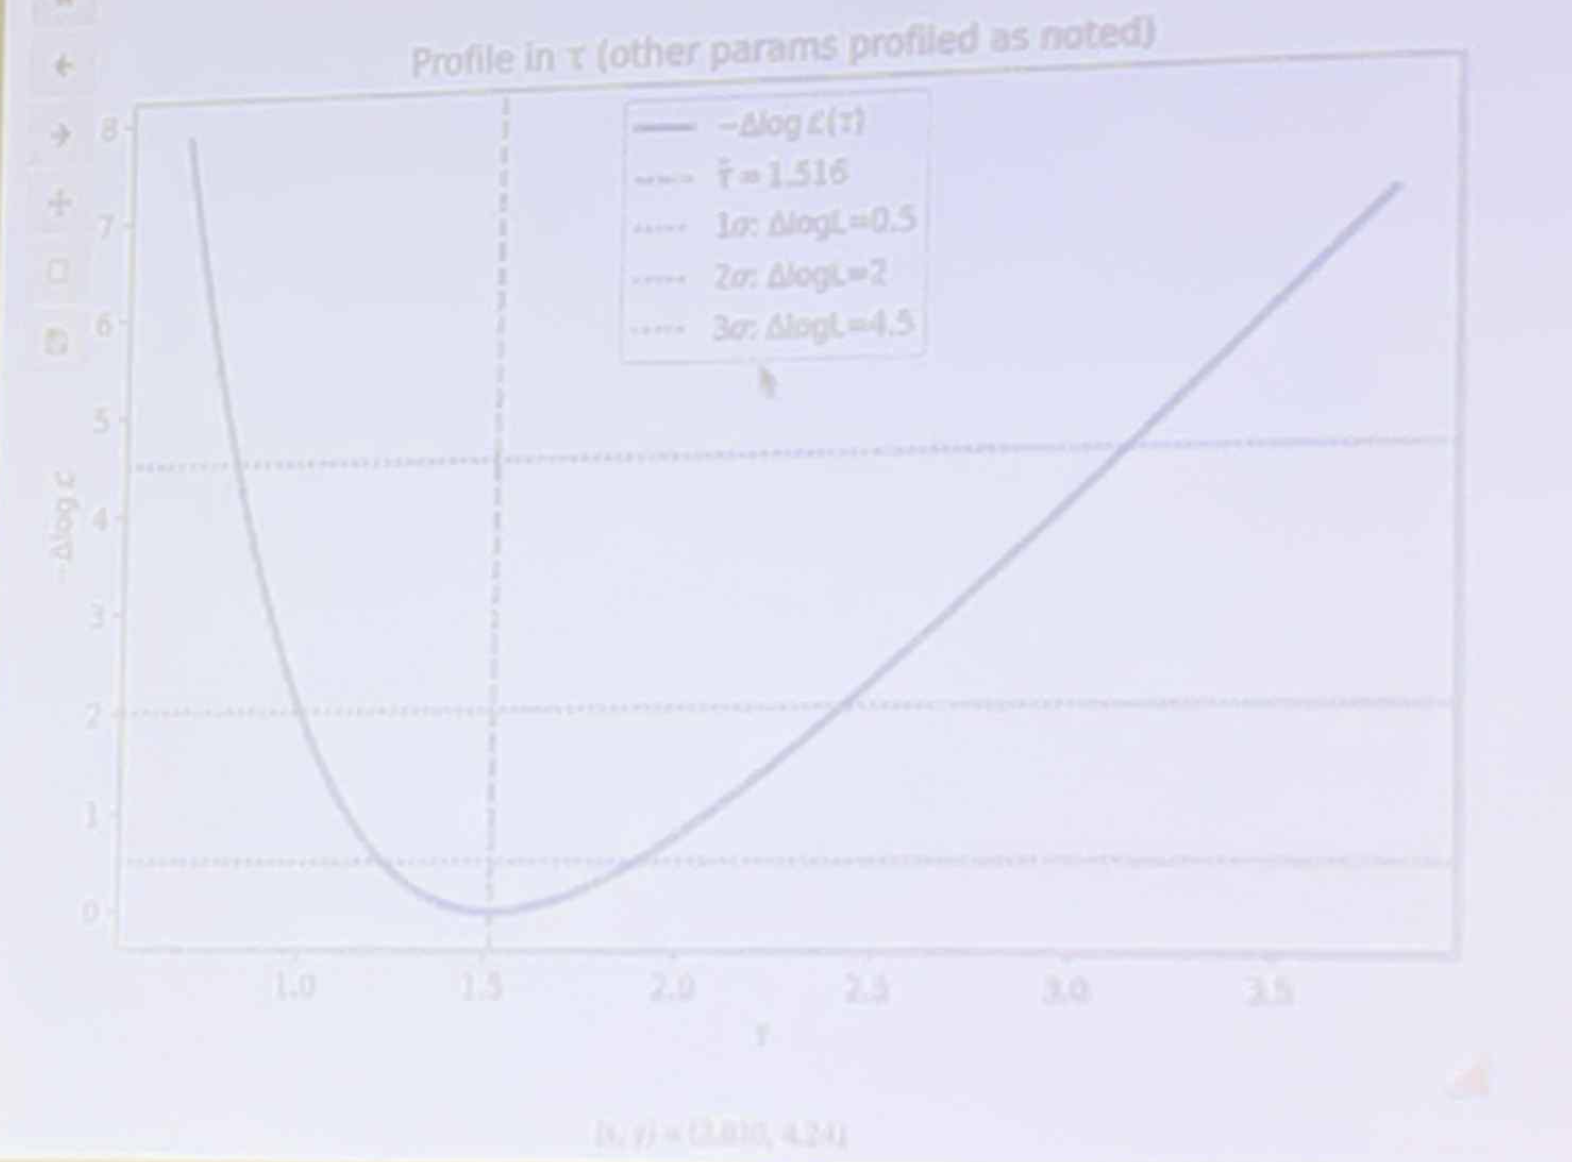
\includegraphics[width = 0.5\linewidth]{Images/lec14-tau-likelihood.png}

            \subsection{Likelihood versus Chi-Squared Interpretation}
      \item Maximum Likelihood is only a function of the shape of your data and whether it matches your model.
      \item $\chi^2$ is a function of both the height and the shape of your data.

            \subsection{Normalization and Extended Likelihood}
      \item We can incorporate the number of data events:
            \[
                  \int P(x|a) dx = 1 \, \forall a
            \]
      \item Define $Q$ such that:
            \[
                  \int Q(x|a) dx = L(a)
            \]
      \item Example: number of muons from cosmic rays passing through counters.
      \item Extend likelihood:
            \[
                  \mathcal{L} = \frac{e^{-\nu} \nu^n}{n!}
            \]
      \item This is called the extended likelihood and contains the Poisson term.
            \[
                  \ln{\mathcal{L}} = \sum_{i} \ln(p(x_i|a)) - \nu - n \ln \nu + \cancelto{0}{\ln n!}
            \]

            \subsection{Nuisance Parameters and Systematic Effects}
      \item Nuisance parameters often represent systematic effects or resolution uncertainties:
            \[
                  \mathcal{L}(\theta) = \mathcal{L}_{0} \frac{1}{\sqrt{2 \pi} \sigma_{\theta}} \exp \left( -\frac{(\theta - \mu)^2}{2 \sigma_{\theta}^2} \right)
            \]
      \item $\theta \sim \mathcal{N}(\mu, \sigma_{\theta}^2)$ is a nuisance parameter.

            \subsection{Gaussian Data Likelihood and Chi-Squared Minimization}
      \item Suppose we have data points of the form $\{ x_i, y_i \pm \sigma_i \}$ and $y_i$ are Gaussian.
      \item We think we know  $y(x) = f(x|a)$.
            \[
                  p(y_i|a) = \frac{1}{\sqrt{2 \pi} \sigma_i} \exp \left( -\frac{(y_i - f(x_i|a))^2}{2 \sigma_i^2} \right)
            \]
            \[
                  \mathcal{L} = \prod_{i} p(y_i|a)
            \]
            \[
                  \ln \mathcal{L} = -\frac{1}{2} \sum_{i} \left( \frac{y_i - f(x_i|a)}{\sigma_i} \right)^2 + \text{const}
            \]
      \item Maximizing $\ln \mathcal{L}$:
      \item Minimizing $\chi^2$:
            \[
                  \chi^2 = \sum_{i} \left( \frac{y_i - f(x_i|a)}{\sigma_i} \right)^2
            \]
      \item i.e. Maximizing likelihood is equivalent to minimizing $\chi^2$ for Gaussian data.

            \subsection{Introduction to Hypothesis Testing}
      \item Next: Hypothesis Testing.
      \item A simple hypothesis is one for which the test statistic has a completely specified pdf.
      \item Example: data come from Poisson process with mean $\nu = 5$–$6$.
      \item A composite hypothesis is one for which the test statistic has a pdf that depends on unknown parameters.

      \item Here is a similar example diagram from the internet:

            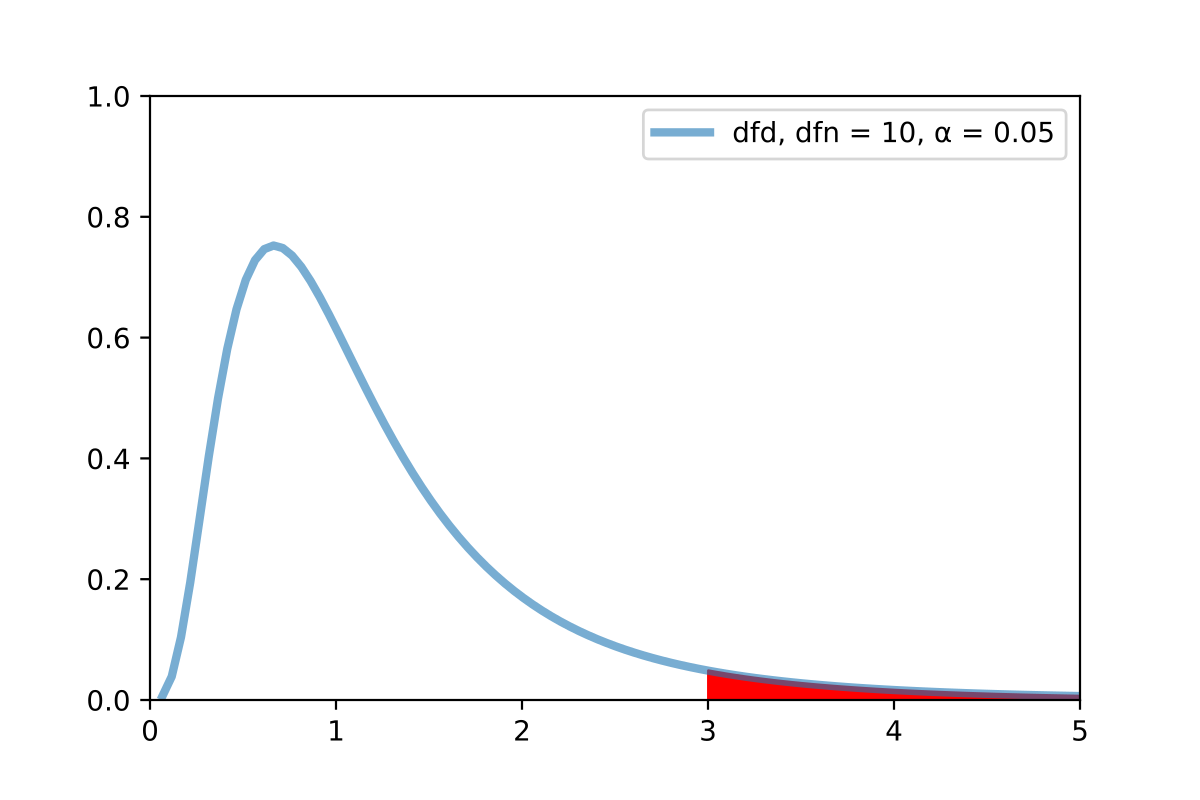
\includegraphics[width = 0.5\linewidth]{Images/lec14-ftest.png}

            \subsection{Rejection Regions and Type I Error}
      \item Decide in advance a $\sigma_i^2$ region of $x$. Reject $H_0$ if $x$ is in this region.
            \[
                  \int_{\text{region}} p(x|H_0) dx = \alpha = \text{significance of test}
            \]
      \item For $x \ge x_0$: “Reject” $H_0$ when true occurs $\alpha$ fraction of the time.
      \item Type I error: Reject $H_0$ when true (probability $\alpha$).
      \item Fisher.
      \item $H_0 =$ Data is $\sim \mathcal{N}(\mu_0, \sigma_0^2)$.
      \item Get pairs $x_1, \, x_2$.
      \item Your choice of possible regions is huge and can lead to very weird tests.

            \subsection{Neyman–Pearson Lemma and Type II Error}
      \item Neyman–Pearson: fixed by adding second hypothesis $H_A$.

            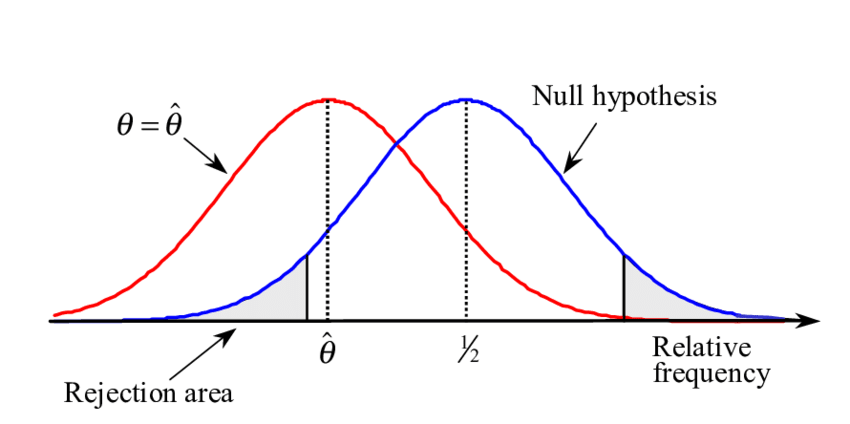
\includegraphics[width = 0.5\linewidth]{Images/lec14-neyman-pearson-test.png}

      \item $\beta =$ power of test.
      \item Only two choices: $H_0$ or $H_A$.
      \item Type II error: Accept $H_0$ when false (probability $\beta$).

            \subsection{Likelihood Ratio Test and Interpretation}
      \item Law: Null hypothesis $H_0$ is rejected in favor of alternative hypothesis $H_A$ if
            \[
                  \Lambda(x) = \frac{\mathcal{L}(x|H_A)}{\mathcal{L}(x|H_0)} \ge k_{\alpha}
            \]
      \item In legal terms: $H_0 =$ innocent until proven guilty, $H_A =$ guilty.
      \item In science: $H_0 =$ no new physics, $H_A =$ new physics.

\end{itemize}
